\documentclass{neu-assignment}


\usepackage{lipsum}
\usepackage{graphicx}
\usepackage{pdfpages}
\usepackage[font=small]{caption}
\usepackage{hyperref}

 

\newcommand*{\name}{Sagar Kumar}
%\newcommand*{\id}{000000000}
\newcommand*{\course}{Complex Networks 2}
\newcommand*{\assignment}{Assignment 1}


\begin{document}

\maketitle


%%%%%%%%%%%%%%%%%%%%
\subsection*{Problem 1} 
%%%%%%%%%%%%%%%%%%%%
\begin{table}[h]
    \centering
    \begin{tabular}{c | c | c | c}
     & $p_n = p \in (0,1)$ & $p_n = \alpha n^{-\beta}$  &  $p_n = \alpha n^{-1}$\\
     \hline
     $\bar{k}$ & dense &  sparse & ultrasparse\\
     $\bar{d}$ & ultrasmall & small & small \\
     $\bar{c}$ & strong & no & no\\
    \end{tabular}
    \caption{Sparsity, described by the behavior of average degree $\bar{k}$ as $n \to \infty$, small-worldness, described by the behavior of average distance between nodes $\bar{d}$ as $n \to \infty$, and clustering, described by the behavior of average clustering, $\bar{c}$ as $n \to \infty$ for three constructions of Erdo\"s-Re\'nyi graphs based on different edge probabilities.}
    \label{tab:my_table}
\end{table}

Table \ref{tab:my_table} describes the sparsity, small-worldness, and clustering of three $G(n,p)$ graphs defined by some $p=p_n$ which is graph-size-dependent. 
\subsubsection*{Sparsity}
To begin, we consider the case of $p_n = p \in (0,1)$. We know that for $G(n, p_n)$, the $P[(i,j) \in E]$ is independent and depends only on p for all nodes $i,j$ and some set of edges $E$ in $G$. Thus, 
\begin{equation}
    \bar{k} = p_n(n-1)
    \label{eq: av_deg}
\end{equation}
Substitution into Eq. \ref{eq: av_deg} the first connection probability, we get $\bar{k}=p(n-1)$ and thus, $\bar{k} \sim n$ and is therefor \textit{dense} in our definitions. 
\par
Doing the same with the second connection probability, we see that $\bar{k} = \alpha n^{-\beta}(n-1) \approx \alpha n^{1-\beta}$. As $\beta \in (0,1)$ by definition, this graph scales as $\bar{k} << n$ to $\bar{k} < n$. Thus, by our definition, this is a \textit{sparse} graph.
\par
Finally, substituting our last value of $p_n$ into Eq. \ref{eq: av_deg}, we get $\bar{k} = \alpha n^{-1}(n-1) = \alpha(1 - 1/n)$. As the last term gets dropped in the thermodynamic limit, $\bar{k} \sim \alpha$ and is thus \textit{ultrasparse} in our definitions. 

\subsubsection*{Small-worldness}

For constant $p$, as in the first case of $p_n = p$, we know that the diameter $\bar{d} \sim 1$. As the definition of small world is 
\begin{equation}
    \texttt{G is small world} \Longleftrightarrow \bar{d} << n^\epsilon\ \forall  \epsilon.
    \label{eq:def_small}
\end{equation}
\begin{equation}
    \texttt{G is ultrasmall} \Longleftrightarrow \bar{d} << \ln^\epsilon(n)\  \forall \epsilon.
    \label{eq:def_ultrasmall}
\end{equation}
As $1 << \ln^\epsilon(n)$ as $n \to \infty$, we classify $G(n, p_n = p\in(0,1))$ to be ultrasmall world.
\par
For the second case, we consider that $\bar{k} \sim n^\epsilon, \epsilon >0$ as per the derivation above. Thus, we know that the average distance is
\begin{equation}
    \bar{d} \sim \frac{\log(n)}{\log(\bar{k})}
    \label{eq:dist}
\end{equation}. 
Substituting our value for $\bar{k}$, we get $\bar{d} \sim \frac{\log(n)}{\log(\alpha n^{1-\beta})} = \frac{\log(n)}{\log(\alpha) + \log(n) - \beta\log(n)}$ the right hand side is therefor $c < \bar{d} < c\log{n}$ where c is some constant factor. Thus, this does not satisfy Eq. \ref{eq:def_ultrasmall} but suffices to satisfy Eq. \ref{eq:def_small} and is thus a small world. 
\par
Finally, we examine the final case in which we know $\bar{k} ~ \alpha > 1$. Thus, from Eq. \ref{eq:dist}, we know that $\bar{d}/\log(n) \to 1/\alpha$ and this is thus a small world as well. 
\subsubsection*{Clustering}
We consider any clustering that is non-zero in the limit to be "strong" clustering. 
For a single node $i$, the clustering coefficient $c_i$ is defined as 
\begin{equation}
    c_i = t_i/w_i
    \label{eq:local_clustering}
\end{equation}
where $w_i$ is the number of pairs of neighbors of a node, and $t_i$ is the number of connected pairs of neighbors. The average clustering $\bar{c}$ which we are looking for is a weighted linear combination of these $c_i$.
However, if we use consider our Erdo\"s-Re\'nyi model to generate graphs, we can see that for any node $i$, Eq. \ref{eq:local_clustering} can be expressed as 
\begin{equation}
    c_i = p_n^3/p_n^2
    \label{eq:ER-clustering}
\end{equation}
From Eq. \ref{eq:ER-clustering}, it is clear that due to the $n$-dependence for our latter two cases, this $c_i$ term completely vanishes to 0. Only in the case of constant $p_n = p$ does a term remain in the thermodynamic limit and thus that is the only graph realization in which we would witness strong clustering. 


%%%%%%%%%%%%%%%%%%%%
\subsection*{Problem 2}
%%%%%%%%%%%%%%%%%%%%

All code for this section is attached but can also be found \href{https://github.com/sagarkumar16/complex-networks-2/blob/main/HW1/HW1.ipynb}{on my Github}\footnote{https://github.com/sagarkumar16/complex-networks-2/blob/main/HW1/HW1.ipynb}.

\subsubsection*{Log-Binning Distribution} See function \texttt{distributionBin()}
\subsubsection*{Log-Binning Function} See function \texttt{functionBin()}
\subsubsection*{Graph Generation} See function \texttt{simpleSF()}
\subsubsection*{Measuring Graph Properties}

\begin{figure}[h!]
    \centering
    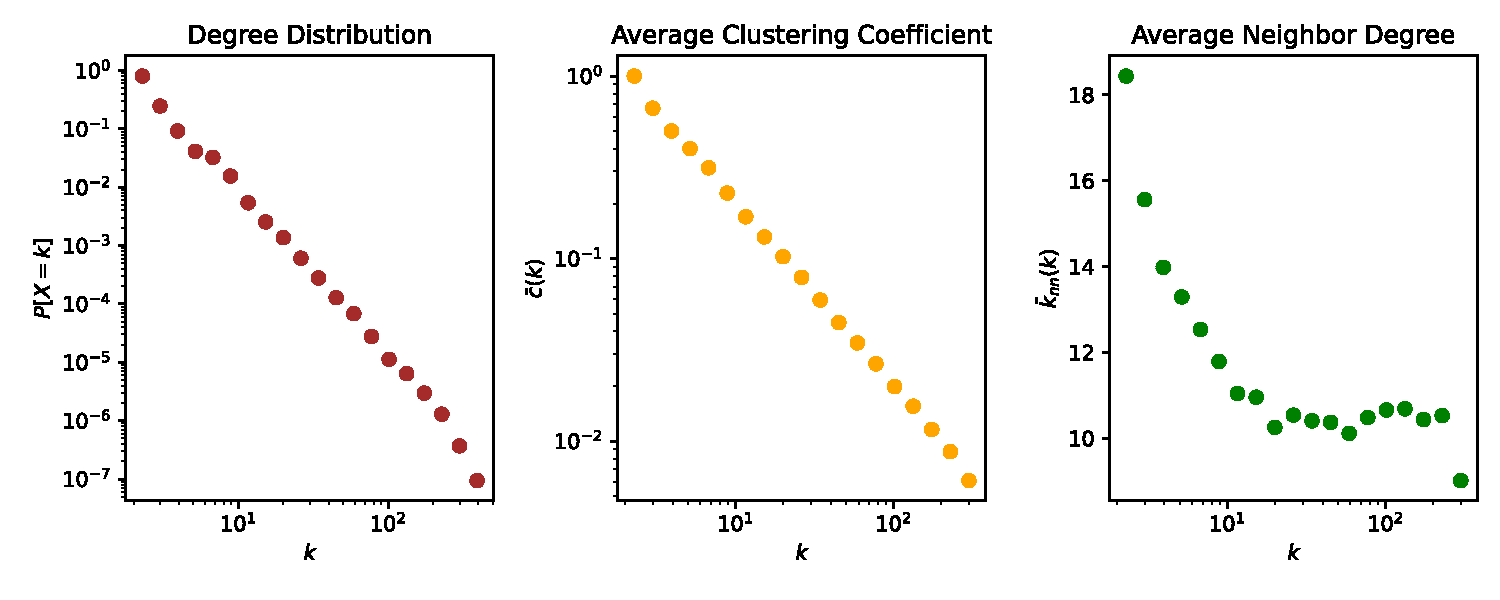
\includegraphics[scale=0.5]{figures/HW1_fig1_pk_ck_knnk.pdf}
    \caption{For the ensemble of $N=10$ graphs of size $n=10^4$ generated using the \texttt{simpleSF()} function: (left) Degree Distribution $P[X=k]$ or $P(k)$ plotted on a log-log scale as a logarithmically binned distribution, (center) Average Clustering Coefficient $\bar{c}(k)$ plotted against degree on a log-log scale, binned logarithmically, and (right) Average Neighbor Degree $\bar{k}_{nn}(k)$ plotted against degree as a logarithmically binned function on a semi-log plot.}
    \label{fig:deg_clu_knnk}
\end{figure}

Figure \ref{fig:deg_clu_knnk} shows the measurements of $P(k), \bar{c}(k), and \bar{k}_{nn}(k)$ for the ensemble of graphs created by the simple Scale-Free graph generation algorithm. For each measurement, all values from each of the graphs was concatenated into a single sequence of values or single sequence of input-output pairs. Thus, the results are the not the measurements for any single of the graphs output nor is it the average of all of them, but rather, a concatenation of all of them. 

The results are consistent with the literature on scale-free graphs. When logarithmically binned, the degree distribution shows a clear power law, as does the average clustering. Average neighbor degree seems to show some signs of "disassortivity" at first, but quickly becomes quite neutral, suggesting that this apparent negative degree assortativity is likely to be a finite-size effect. 

\begin{figure}[h!]
    \centering
    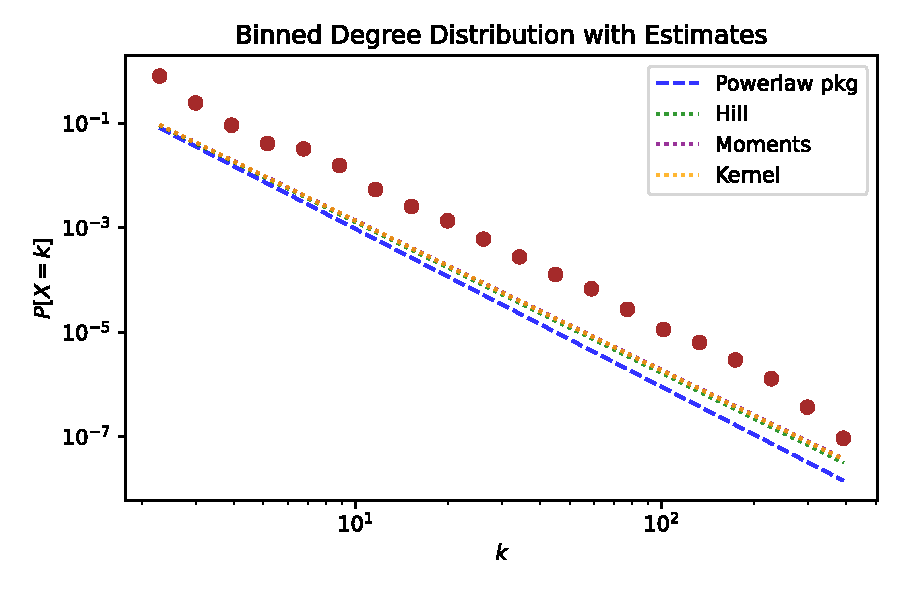
\includegraphics[scale=0.7]{figures/HW1_fig2_degree_dist_estimates.pdf}
    \caption{The degree distribution as shown in Fig. \ref{fig:deg_clu_knnk} plotted alongside estimates from the \texttt{powerlaw} package, as well as the Hill, Moments, and Kernel estimates from \textit{Tail Index Estimation for Degree Sequences of Complex Networks}\footnote{https://github.com/ivanvoitalov/tail-estimation}}.
    \label{fig:etimation}
\end{figure}

\begin{table}[h!]
    \centering
    \begin{tabular}{c c}
        Estimator  &  $\gamma$ \\
        \hline
        \texttt{powerlaw} & 3.022 \\
        Hill & 2.890 \\
        Moments & 2.860 \\
        Kernel & 2.865
    \end{tabular}
    \caption{Summary of rounded estimations for the exponent, $\gamma$, on a power-law fit of the degree distribution}
    \label{tab:estimates_table}
\end{table}

Figure \ref{fig:etimation} shows estimates from the \texttt{powerlaw} package, as well as Hill, Moments, and Kernel estimates of the same degree distribution plotted in Figure \ref{fig:deg_clu_knnk}. Table 2 provides the $\gamma$ estimates, rounded after 3 decimal points. Clearly, there is some spread in these estimates. Interestingly, the \texttt{powerlaw} package, unlike the other estimators, place this graph in the regime of $\gamma > 3$ and visually, seems to diverge further fro the true value than the other estimates which have been proven to be optimal and consistent. Nevertheless, all estimators are in consensus that this model does indeed have a diverging second moment in the infinite limit and is thus scale-free. 

\subsection*{Appendix: Code}
\includepdf[pages=-]{HW1_DS_PDF.pdf}


\end{document}

% PL: 3.02235200896027
%Adjusted Hill estimated gamma: 2.889644431436195
%%Moments estimated gamma: 2.8602879353057453
%Kernel-type estimated gamma: 2.8648694044336103